\chapter{Diagrama de estado}
\addcontentsline{toc}{chapter}{Diagrama de estado}

Apresentação dos estados de uma entidade de medida que foi capturada ao longo da interação com o sistema.

\begin{figure}[H]
    \label{figure_diagrama_estado}
    \centering
    \caption{Diagrama de estado}
    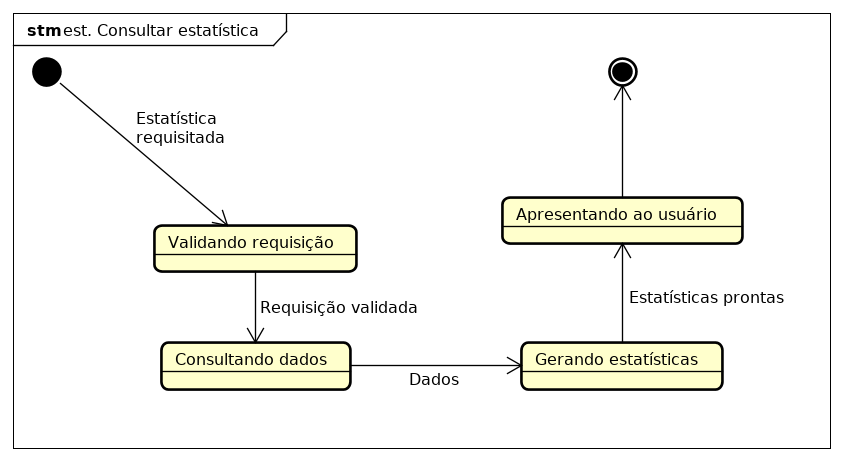
\includegraphics[scale=0.6]{diagrams/estado.png}
    \hfill
\end{figure}

Conforme descrito na figura \ref{figure_diagrama_estado} os estados durante o armazenamento de uma de uma medida são:

\section{Validando requisição}

A autenticação do arduino na API foi feita e a requisição HTTP para o armazenamento de uma medida foi feita até a API.
Nesse estado, a requisição está passando por uma validação básica, verificando os tipos e formato dos dados.

\section{Validando regras de negócio}

A medida passou pelo controlador e está sendo validada através dos filtros, onde as regras de negócio de validação estão verificando se aquela medida faz sentido, baseando-se nas medidas captadas anteriormente.

\section{Armazenando em banco de dados}

A medida é valida e está sendo armazenada no banco de dados, após, ela é retornada a camada de serviço.
